\documentclass[twoside,numberorder]{csbachelor}

%==============================================================
%==============================================================

\usepackage{url}
\usepackage{subfigure}

% 张海:其他引用
\usepackage[hidelinks]{hyperref}
\usepackage{pdfpages}

% 一些全局工具的定义
\DeclareMathOperator*{\argmin}{arg\,min}
\DeclareMathOperator*{\argmax}{arg\,max}

%==============================================================
%==============================================================

\begin{document}

\pagestyle{empty}

%==============================================================
%==============================================================

  % 论文题目:{中文}{英文}
  \zjutitle{在线交互式神经元重建的服务器系统}
           {todo}
  % 作者:{中文姓名}{英文}{学号}
  \zjuauthor{曲衡}{Heng Qu}{3130000569}
  % 指导教师:{导师中文名}{导师英文名}
  \zjumentor{郑能干}{Nenggan Zheng}
  % 个人信息:{年级}{专业名称}
  \zjuinfo{2013级}{计算机科学与技术}
  % 学院信息:{学院中文}{学院英文}
  \zjucollege{计算机科学与技术学院}{College of Computer Science and Technology}
  % 日期:{Submitted Date}
  %\zjudate{2017-03-29}

%==============================================================

  \thispagestyle{empty}

{
\setlength{\parindent}{0em}
\renewcommand{\baselinestretch}{2}

\vspace*{-7mm}

\begin{center}
  
\includegraphics[width=108mm]{data/cover/xiaoming}
\end{center}

\vspace{-1mm}

{
\renewcommand{\baselinestretch}{1.8}
\heiti\erhao\bfseries
\centering
本~~科~~生~~毕~~业~~设~~计 \\
中期报告 \par
}

\vspace{4em}

\begin{center}
  
\includegraphics[width=35mm]{data/cover/xiaobiao}
\end{center}

\vspace{3em}

{
\renewcommand{\baselinestretch}{1.65}
\songti\sanhao\bfseries
\centering
题目 \; \underline{\makebox[16em]{\zjutitlec}} \\
姓名 \; \underline{\makebox[16em]{\zjuauthornamec}} \\
学号 \; \underline{\makebox[16em]{\zjuauthorid}} \\
指导教师 \; \underline{\makebox[14em]{\zjumentorc}} \\
年级与专业 \; \underline{\makebox[13em]{\zjugrade~~\zjumajor}} \\
所在学院 \; \underline{\makebox[14em]{\zjucollegec}} \par
}
}

\ifthenelse{\equal{\zjuside}{T}}{\newpage\mbox{}\thispagestyle{empty}}{}


  \newpage

\thispagestyle{empty}

{
\setlength{\parindent}{0em}
\renewcommand{\baselinestretch}{2}
\songti\sihao\bfseries

一、 \; 题目: \; \underline{\makebox[24em]{\zjutitlec}}

\vspace{2em}

二、 \; 指导教师对开题报告、外文翻译和中期报告的具体要求:

1. \; 开题报告要求: \; 要求。

2. \; 外文翻译要求: \; 要求。

3. \; 中期报告要求: \; 要求。

\vspace{8cm}
}

{
\songti\xiaosi\bfseries
\begin{flushright}
  指导教师(签名) \; \underline{\hspace{6em}} \\
  年 \qquad 月 \qquad 日
\end{flushright}
}

\ifthenelse{\equal{\zjuside}{T}}{\newpage\mbox{}\thispagestyle{empty}}{}


  \thispagestyle{empty}

{
  \setlength{\parindent}{0em}
  \renewcommand{\baselinestretch}{2}

  {
    \stfangsong\sanhao\bfseries
    \centering
    毕业设计开题报告、外文翻译的考核 \par
  }

  {
    \songti\sihao\bfseries
    导师对开题报告、外文翻译的评语及成绩评定:

    \vspace{10em}

    {
      \renewcommand{\baselinestretch}{1}

      \begin{flushright}

        \begin{tabular}{|c|c|c|c|}
          \hline
          成绩比例 & \parbox[c]{3.6em}{\xiaosi 开题报告 \\ 占(20\%) \vspace{0.25em}} & \parbox[c]{3.6em}{\xiaosi 外文翻译 \\ 占(10\%) \vspace{0.25em}} \\
          \hline
          分值 & & \\
          \hline
        \end{tabular}

        \vspace{2em}

        {
          \songti\xiaosi\bfseries
          导师签名 \; \underline{\hspace{6em}} \\
          年 \qquad 月 \qquad 日 \par
        }
      \end{flushright}
    }
  }

  \vspace{2em}

  {
    \songti\sihao\bfseries
    学院盲审专家对开题报告、外文翻译的评语及成绩评定:

    \vspace{10em}

    {
      \renewcommand{\baselinestretch}{1}

      \begin{flushright}

        \begin{tabular}{|c|c|c|c|}
          \hline
          成绩比例 & \parbox[c]{3.6em}{\xiaosi 开题报告 \\ 占(20\%) \vspace{0.25em}} & \parbox[c]{3.6em}{\xiaosi 外文翻译 \\ 占(10\%) \vspace{0.25em}} \\
          \hline
          分值 & & \\
          \hline
        \end{tabular}

        \vspace{2em}

        {
          \songti\xiaosi\bfseries
          开题报告审核负责人(签名/签章) \; \underline{\hspace{6em}} \par
        }
      \end{flushright}
    }
  }

  \newpage

  {
    \stfangsong\sanhao\bfseries
    \centering
    毕业设计中期报告考核 \par
  }

  {
    \songti\sihao\bfseries
    导师对中期报告的评语及成绩评定:

    \vspace{10em}

    {
      \renewcommand{\baselinestretch}{1}

      \begin{flushright}

        \begin{tabular}{|c|c|c|c|}
          \hline
          成绩比例 & \parbox[c]{3.6em}{\xiaosi 中期报告 \\ 占(10\%) \vspace{0.25em}} \\
          \hline
          分值 & \\
          \hline
        \end{tabular}

        \vspace{2em}

        {
          \songti\xiaosi\bfseries
          导师签名 \; \underline{\hspace{6em}} \\
          年 \qquad 月 \qquad 日 \par
        }
      \end{flushright}
    }
  }
}


  \tableofcontents
  \thispagestyle{toc}
  %\chaptermark{目录}

  \mainmatter

  {
    \pagestyle{kaitibaogao}
    \makeatletter
      \let\ps@plain\ps@kaitibaogao
    \makeatother
    \chapter*{\zjutitlec 开题报告}

\section{项目背景}
将原始神经元图像信息进行神经元追踪和数字重建,有助于神经科学家直观地观察神经元结构,理解大脑运作的原理,甚至于探索智能的起源。因此,对大脑神经元相互连接形成的复杂网络进行数字重建一直是大脑神经科学家的目标之一。最近在神经元拓扑结构的自动化数字重建算法上取得了一些进展,如 Cannon RC 等人在海马神经重建上做出的工作\cite{Cannon1998An},Feng L 等人使用 mGRASP 在鼠类大脑上进行的重建工作\cite{Druckmann2014Structured}均取得了出色的进展。

由于神经元拓扑结构的复杂性,在一些自动化重建结果的细节上仍然需要研究人员对数字重建的结果进行人工纠正和修改,以确保数字重建工作的准确性。另外研究人员需要对数字重建结果进行编辑,比如添加或删除一些网络分支等。为了便于研究人员编辑数字重建的结果,根据“所见即所得”的原则,设计出了 SWC 格式\cite{Peng2011Proof}。SWC 框架有以下特征: 清楚的 SWC 结构以及原始数据参考的可视化,明确定义的可操作单元,以及将用户输入和编辑操作直观地对应起来。在 SWC 格式的基础上,研究人员可以方便、直观地纠正自动化数字重建结果的错误,添加新的分支或删除已有分支。

尽管在 SWC 格式的基础上已经开发出了大量可以产生 SWC 格式文件的神经元结构重建软件,例如专注于半自动重建的 FARSIGHT \cite{Luisi2011The}、半手动半自动重建的 Neuromantic \cite{Myatt2012Neuromantic},以及一些其他主流数字重建工具 Vaa3D \cite{Peng2010Seeing}、Neurostudio \cite{Rodriguez2006Rayburst} 等等。但是这些软件并没有充分利用 SWC 格式的优点,并且为用户提供高效、精确重建的界面,在 \cite{Feng2014neuTube} 中对这些软件的优缺点进行了详细的论述。为了充分发挥 SWC 格式高效,精确的优点,提供一个学习成本低,操作直观,并能提供相应的数据可视化功能,赵挺老师基于 SWC 格式,设计了名为 neuTube 的新软件\cite{Feng2014neuTube},同时具备 2D 和 3D 的可视化和直观的编辑、绘制功能。

由于 neuTube 是运行在单机的软件,无法满足多用户协同编辑修改的需求,也不利于数字重建结果的交流,无法共享完成数字重建的神经元结构。随着计算机性能和网速的提升,使得在线实时编辑神经元网络结构成为了可能。在此背景下,我们希望设计并实现一个在线多用户的神经元网络结构编辑平台,利用互联网便于数据共享的特点,帮助神经学研究人员便捷地进行异地,多用户协同编辑神经元网络结构,并能分享完成数字重建的神经元结构,共同探索神经元结构下的奥秘。

\section{目标和任务}
\subsection{目标}
我们的目标是设计并实现在线多用户的神经元网络结构编辑平台,利用互联网数据共享的特点,帮助神经学研究人员可以进行异地,多用户协同编辑神经网络结构,并能分享人工纠正、修改得到的神经元结构。充分发挥 SWC 文件格式准确,清楚,高效的优势,提供一个便于交互,同时具备 2D 和 3D 的可视化和直观的编辑、绘制功能的在线多用户神经网络结构编辑平台,并能处理多用户同时编辑时可能产生的冲突。

在这个平台上,用户可以上传神经回路的原始图像信息并储存在云端的服务器之中,利用 neuTube 或自己实现神经元网络结构的自动化数字重建工作。使用 SWC 格式储存数字重建工作的结果,作为后续修改、编辑的基础。平台包含数据可视化的功能,将数字重建结果以 2D 和 3D 的形式展现给用户。用户可以对数字重建结果进行人工编辑、修改,纠正自动数字重建结果中不精确的细节。用户也可以在已经完成的数字重建结果的基础上,删除已有分支或添加新的分支。

由于允许多用户同时编辑同一份 SWC 文件,这可能会造成文件内容的冲突。我们需要提供一套文件冲突解决方案,在文件内容产生冲突的时候尽可能地自动解决冲突,并能将实在解决不了的冲突准确、直观的表述给用户,便于用户手动解决冲突。

\subsection{任务}
设计完成上述需求的神经元网络结构编辑平台,将原始神经元图像信息应用于本平台,由神经科学家通过本平台编辑,修改完成数字重建的神经元结构,并根据反馈提高平台的可用性。
对系统的要求:

1. 交换界面简洁明了,操作简洁高效

2. 对多用户协同编辑提供支持

3. 能够解决多用户协同编辑产生的冲突

4. 用户操作延迟较低,没有明显的卡顿

\section{可行性分析}
郑能干老师和赵挺老师作为指导老师,在神经网络结构重建与编辑领域具有多年的工作经验,提供了清晰、明确的工作方向,在可能遇到问题的地方提供指导和帮助,为解决潜在的问题提供了保障。neuTube 作为已经实现的单机版本,明确了项目需求,展示出一些可能存在的问题,使我对该项目的理解更加深入透彻。技术方案里面涉及的很多技术是由赵挺老师所在实验室开发的,甚至是由赵挺老师本人编写完成的。两位指导老师提供的技术指导大大提高了项目可行性。

项目组积累了大量原始神经元切片图像数据,有充分的测试数据完成平台设计与开发。

项目前期对项目可能涉及到的技术做了充分的研究,尝试,对顺利完成项目内容,达成项目目标有充分的信心。

由于本项目不涉及硬件方面,项目经费需求较小。项目涉及到的服务器和开发平台均能利用现有实验室资源完成,可行性较高。

\section{初步技术方案和关键技术考虑}
技术方案涉及原始图像信息储存与数字重建结果储存,用户数据信息储存,网络应用开发以及前端可视化展示,共4个部分。

\subsection{原始图像信息与数字重建结果储存}
我们初步计划采用 DVID 储存原始图像信息与数字重建结果。DVID 是一个分布式面向图像的数据服务,主要用于图像分析与可视化。DVID 有如下特点:

1. 便于扩展数据类型,允许用户根据数据特点加速访问速度,减少储存空间,提供方便的 API。这为储存数字重建结果提供了便利。

2. 为分布式数据储存提供了类似于 GIT 的版本控制系统,在此基础之上我们可以解决多用户同时编辑产生冲突的问题。

3. 方便连接其他 API 如 Google BrainMaps 和 OpenConnectome 等。

4. 支持多分辨率图像数据,使得用户可以在不同尺度下观察图像信息。

在 DVID 的基础上,可以构建出多用户的原始图像信息与数字重建结果储存仓库,将数据储存抽象成数据存储服务,便于专注于完成核心算法和逻辑。

\subsection{用户数据信息储存}
初步计划采用 PostgreSQL 数据库储存用户信息。PostgreSQL 最初由加州大学伯克利分校计算机系开发完成。在支持大部分 SQL 标准之上,提供了许多诸如复杂查询,多版本并行控制,事物完整性等现代特性。由于 PostreSQL 对标准 SQL 支持度较高,可以方便的和 DVID 联系起来,将用户信息和原始图像信息,数字重建结果对应起来。利用 PostgreSQL 支持的储存过程,事物以及多版本并行控制特性,我们可以方便的实现分布式,多用户实时编辑平台,并解决多用户同时编辑可能产生冲突的问题。

\subsection{网络应用开发}
初步计划采用 Node.js 和 Express 完成网络应用开发。
Node.js 是一个基于 Chrome V8 引起的 JavaScript 的运行环境。Node.js 使用了一个事件驱动、非阻塞式 I/O 的模型,使其轻量又高效。Express 是一个基于 Node.js 平台的极简、灵活的 web 应用开发框架,提供丰富的 HTTP 快捷方式和任意排列组合的 Connect 中间件,帮助快速、简单的创建健壮、友好的 API。
\begin{figure}
\centering
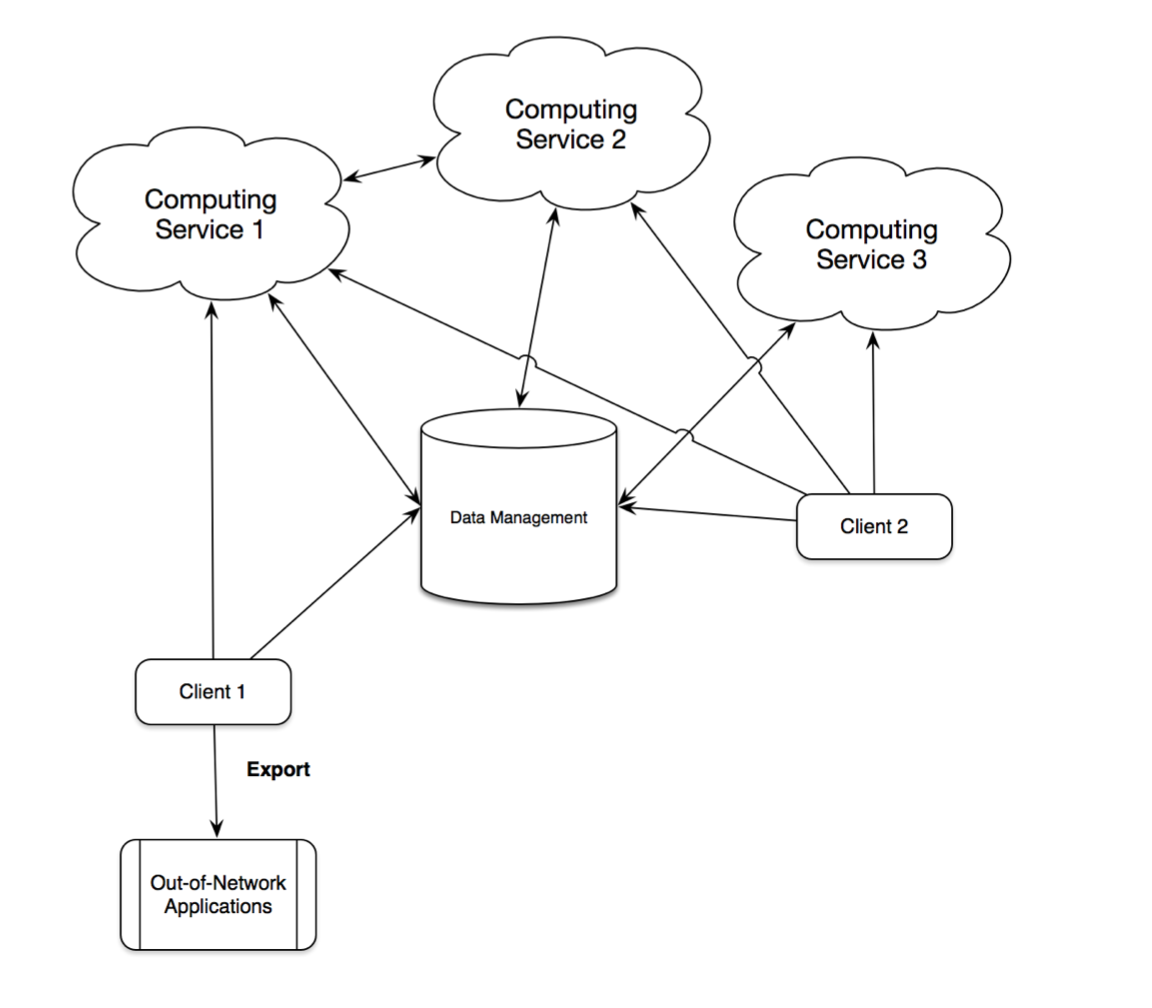
\includegraphics[width=108mm]{images/server}
\caption{分布式计算服务结构}
\label{server}
\end{figure}
基于这两个工具,可以方便快速的搭建一个无状态的服务器,初步设计出一个分布式计算服务结构如图 \ref{server} 所示,便于针对用户数量以及数据请求量进行扩展。搭配之前采用的分布式数据库,网络应用平台的可扩展性较高,可以用来应对多用户同时编辑大数据量的数据,并提供相应可视化算法所需的计算服务的应用场景。

\subsection{前端可视化展示}
这部分工作主要由同组其他同学完成,主要用到的技术有 Three.js 和 React 等, 这里不再赘述。 

\section{预期工作结果}
1. 神经元结构编辑平台

设计并实现一个同时具备 2D 和 3D 的可视化界面,为用户提供直观的编辑、绘制功能,支持多用户同时在线并可以协同编辑的神经元结构平台。实验室其他同学完成数据可视化工作,我主要实现平台的后端支持。

2. 同时在线用户数测试报告

对神经元结构编辑平台进行压力测试,根据测试结果进行性能调优,使之支持尽可能多的同时在线用户数量(数千用户同时在线,取决于平台后端计算机的性能和数量)。完成性能调优后提供一份完整的性能测试报告。

3. 用户操作延迟测试报告

对前端可视化操作的响应时间进行压力测试,根据测试结果进行性能调优,使用户操作的响应时间在毫秒级别(大量数据的上传时间取决去客户端所处网络环境)。对各个操作的响应时间及优化结果提供详细的测试报告。


\section{进度计划}

本项目的整体计划如下表所示:

\begin{table}[!htbp]
\centering
\begin{tabular}{|l|l|}
\hline
时间 & 主要工作 \\ \hline
2017 年 3 月 1 日 至 3 月 15 日& 完成项目功能点的需求及初步技术方案设计 \\ \hline
2017 年 3 月 16 日 至 3 月 29 日& 完成多用户平台设计 \\ \hline
2017 年 4 月 1 日 至 4 月 15 日& 初步完成需求的功能点 \\ \hline
2017 年 4 月 16 日 至 4 月 30 日& 并根据指导老师意见进行功能迭代,开始撰写论文 \\ \hline
2017 年 5 月 1 日 至 5 月 30 日& 根据测试结果进行性能调优,根据老师意见修改并完成论文 \\ \hline

\end{tabular}
\caption{项目进度计划}
\label{table:schedule}
\end{table}

\bibliographystyle{data/gbt7714-2005}
{
\renewcommand{\chapter}[2]{\section*{#2}\addcontentsline{toc}{section}{#2}}
\bibliography{data/kaitibaogao}
}

% 按文章长度需要启用
\ifthenelse{\equal{\zjuside}{T}}{\newpage\mbox{}\thispagestyle{empty}}{}

  }

  {
    \pagestyle{waiwenfanyi}
    \makeatletter
      \let\ps@plain\ps@waiwenfanyi
    \makeatother
    \setcounter{page}{1}

    \renewcommand{\addcontentsline}[3]{}

    \thispagestyle{empty}
{
\chapter{本科毕业设计外文翻译}

基于 SWC 文件格式的一种高效神经重建的新设计

\section{概要}

大脑回路的绘制需要在神经拓扑形成的复杂网络上进行数字重建。 尽管最近几年在自动化算法上取的了一些进展,由于缺少高效的重建并支持用户编辑的软件, 神经结构的重建依旧是大脑回路绘制的瓶颈。因此我们设计了一种基于 SWC 文件格式的新软件。 SWC 格式是一种被广泛用于分析神经结构或者在线神经重建的标准神经形态学的格式。 我们同时在我们的开源软件 neuTube 1.0 中实现了这种设计。 这个软件同时具备 2D 和 3D 的可视化和直观的编辑、绘制功能, 允许用户有效的根据荧光图像数据重建神经结构并且编辑由其他软件生成的标准的神经结构文件。 通过和其他两种软件工具的比较(Neuromantic 和 Neurostudio)展示出 neuTube1.0 的优点。 这个软件现在可以在http://www.neutracing.com 上获取, 并提供了完整的软件文档和视频教程。

\section{简介}
从光学显微镜图像中进行神经拓扑结构的数字重建或者绘制是大脑回路构建中的重要一步。 在这个任务中,输入是图像信息, 输出通常是可以被 SWC 格式可以描述的树形结构。 尽管已经开发了大量可以产生 SWC 格式文件的神经重建软件,但是没有充分利用 SWC 格式并且为用户提供高效精确重建的界面。一个最优的用户界面意味着用户可以用最小的认知负荷与软件交互,这就需要清楚的数据可视化和直观的操作。换句话说,根据软件提供的视觉信息,用户应该能够迅速找出底层SWC模型,知道如何操作模型并得到操作的结果。有了这些标准,我们可以识别许多绘制软件应用程序的缺点。例如 FARSIGHT 其重点是半自动的重建神经元的结构,不提供直观的低级编辑功能来纠正细小的错误。Simple Neurite Tracer,Fiji的一个流行的插件, 也缺乏编辑功能。主流的商业软件Neurolucida,允许完成手工重建神经元结构的结构。然而它不支持神经元重建的 3D, 尽管 3D 交互可以提高重建过程的速度和准确性。其他受欢迎的软件工具如 Neuromantic 和 Neurostudio, 同样缺乏先进的 3D 编辑功能。Vaa3D 提供创新的交互式 3D 神经元绘制功能, 但是这些功能在 2D 层面用来确定密度或其他细小结构并不可用。

在这里,我们基于SWC格式提出一种新的、综合软件设计用来克服当前软件的多种局限性。在我们称之为 SWC 框架的基础上,我们开发了 NeuTube,一种结合了鲁棒的自动绘制算法的高效的自动重建的软件工具, 提供了通用的用户友好的 2D 和 3D 编辑功能。

\section{材料和方法}

\subsection{SWC 框架}

\begin{figure}
\centering
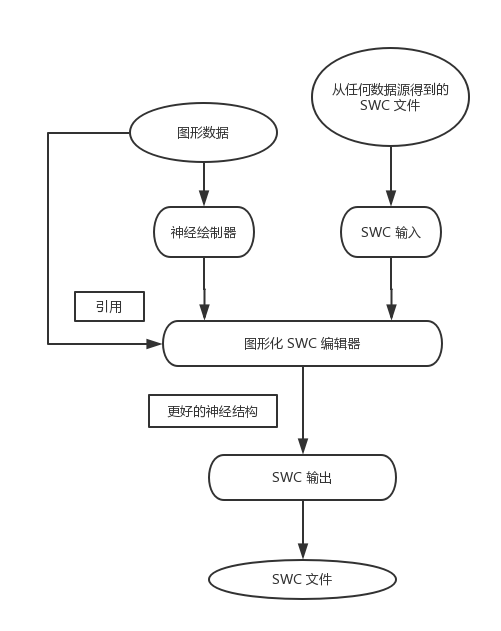
\includegraphics[width=108mm]{images/t1}
\caption{SWC 框架的整体布局}
\label{fan1}
\end{figure}

SWC 框架的整体布局如图 \ref{fan1} 所示。这种结构的软件以原始图像或一个 SWC 文件作为输入,输出的是满足用户需求的神经元结构。SWC 框架遵循的原则是“你所看到的就是你得到的”, 用户正在编辑的结构被可视化出来,检查结果时不需要任何的第三方软件来展示结果。因此,SWC框架包括以下特征: 清楚的 SWC 结构以及原始数据参考的可视化,明确定义的可操作单元,从用户输入和编辑操作直观的对应起来。除了图像可视化,这些特性是建立在 SWC 格式的基础之上。在这里,我们为了详细描述如何构建操作SWC模型,首先用抽象的方式定义了一个模型。

\subsubsection{SWC 模型的抽象定义}

从数学的角度来看,SWC 模型可以用点集来定义:$\{ n_i = (x_i, y_i, z_i, n_j) | i = 1,..., N, j = 0,..., N, i \neq j, x_i, y_i, z_i, r_i \in R \}$ 每一个点 $n_i$, 都是一个中心在 $(x_i, y_i, z_i)$,半径为 $r_i$ 的球。$n_0$ 是一个空点,用来表示一个神经结构的根,$n_j$ 用来表示 $n_i$ 的父节点。 一个向上的路径从 $n_i$ 到 $n_j$ 可以用一个数组 $(n_{k_1},...,n_{k_n})$,其中 $n_{k_i+1}$ 表示 $n_{k_i}$ 的父节点 $k_1 = i, k_n = j$。一个合法的神经树形结构,是不允许有环的存在。在这个模型中,基础结构单元是点,点定义了我们如何设计可视化和交互的方案。

\subsubsection{SWC 操作}
假设 $S_1$ 和 $S_2$ 是两个点集,对于一个神经结构的操作可以定义为:
$$f(S_1) = S_2$$
举例来说,$f(\{n_1,...,n_n \} = \phi), \phi$ 代表空集 定义了删除操作。然而一些操作可能产生一些表示非法神经结构的点集。 如何构造合法的操作取决于如何用合适的数据结构描述模型。在我们的框架中,我么使用冗余的元组来储存点集:$n=(G(n), P(n), C(n), S(n))$, 其中 $G(n) = (x(n), y(n), z(n), r(n))$。这种方式定义了一个在$(x(n), y(n), z(n), r(n))$ 处,半径为$r(n)$,父节点为 $p(n)$ 的节点 $n$。 $n$ 的第一个子节点为 $C(n)$,下一个兄弟节点为 $S(n)$。这样的冗余的设计是为了提高遍历节点的效率。例如,要查询子节点时,该程序只需要检查它的第一个孩子和遍历其兄弟节点即可。而在非冗余结构中,每个节点只与其父节点相连,程序可能需要检查树中的每个节点。

编辑一个节点 $n$ 的值可以用修改对应的元组来定义。我们将对 $G(n)$ 的改变称为几何操作,对 $P(n), C(n), S(n) $ 的变换成为结构操作。 一个几何的变换是很直观的,但是一个在结构上的操作很可能造成非法的神经结构。例如仅改变 $P(n)$ 会打破 $P(C(n)) = n, P(n) = P(S(n))$ 的规则。为了避免这样的问题, 我们在三个层次上构建对 SWC 的操作。 第一级包含三个基本操作, 可以用以下公式定义:
$$f_p(\{n\}|n') = f_p(\{G(n), P(n), C(n), S(n)\}|n' = \{(G(n), n', C(n), S(n))\})$$
$$f_p(\{n\}|n') = f_p(\{G(n), P(n), C(n), S(n)\}|n' = \{(G(n), P(n), n', S(n))\})$$
$$f_s(\{n\}|n') = f_p(\{G(n), P(n), C(n), S(n)\}|n' = \{(G(n), P(n), C(n), n')\})$$
在这个层次上,并不保证结构的合法性。

第二层次包括简单有效的操作。假设 $F_{p_0}(n)$ 代表将节点 $n$ 的父节点设为 $n_0$, 即空节点, 如果$C(P(n)) = n$。即n是父母的第一个孩子。
$$
F_{p_0}(n) =
\left\{
\begin{aligned}
f_s(\{n\} | n_0) \circ f_p(\{n\} | n_0) \circ f_c(\{P(n)\} | S(n)), C(P(n)) = n\\
f_s(\{n\} | n_0) \circ f_p(\{n\} | n_0) \circ f_c(\{S^{-1}(n)\} | S(n)), otherwise
\end{aligned}
\right.
$$
其中,$f \circ g$ 代表一个符合操作,$S(S^{-1}(n)) = n$。为了更清楚的定义一个单节点, 在不增加歧义的情况下,$F_{p_0}(n)$ 被定义为一个函数而不是一个点集。
设置父节点的操作被定义为
$$F_p(n|n') = f_c(\{C(n')\}|n) \circ f_s(\{n\}|C(n'))  \circ f_p(\{n\}|n') \circ F_{p_0}(n)$$
设置 $n$ 作为 $n'$ 的第一个子节点虽然可以用其他的操作合成出来,但是在实践中,定义更多的操作是十分有用的。
$$F_s(n|n') = f_s(\{n'\}|n) \circ f_s(\{n'\}|S(n))  \circ f_p(\{n'\}|P(n)) \circ F_{p_0}(n')$$

第三层次由一组复合操作组成,其中包括任何操作组成的第二层次的操作。在这个层次,我们将操作分为两种类型形态依赖和形态独立。如果操作的结果依赖于节点的位置或尺寸,那么这个操作被称为形态依赖,否则被称为形态独立独立。
将一个操作分解为基本操作有助于保证对神经元结构进行的操作的有效性。更重要的是,分解基础操作有助于实现撤销和重做任意操作。撤销操作要求撤消任意复杂度的操作。例如,删除的逆运算需要恢复多个相邻的节点。直接推导逆操作不仅需要大量的工作,也容易导致很难绘制错误。将一个操作分解为一系列基本操作之后,我们可以很容易构造撤消操作的逆转序列。

\subsubsection{用户交互}
绘制软件基本功能是根据用户的输入改变神经元的形态学结构,这通常是由鼠标点击和键盘输入。因为我们定义的操作为将一组节点映射到另一个节点,用户交互从节点的选择开始,这就需要两个组件:SWC 可视化和对用户输入的响应。高质量的可视化神经元是成功的神经元编辑最重要的特征。查看结构的能力显著减少了检查错误所需要时间。提供 2D 和 3D 视图在不同方面体现了独特的优势。例如,3D 视图非常适合显示一个全球结构,而 2D 视图适合在结构密集的地方的精确显示。
选择一个节点最直观的方法是将鼠标光标移到节点上然后单击。这需要将屏幕光标的坐标映射到 3D SWC 空间。同时应该支持选择一组节点作为一个操作的输入。选择后,用户可以用一些输入触发一个操作。所以操作变成了
$$f(S_1\Theta) = S_2$$
$\Theta$ 指的是用户输入的参数。举例来说, $f(\{n\}|(x, y, z)) = \{n, F_p((x, y, z, r(n)), n_0, n_0, n_0)|n\}$, 定义了从节点 $n$ 扩展一个分支到 $(x,y,z)$。

\subsubsection{从图像信号创建 SWC 节点}
对于任何独立的神经绘制软件软件,必须允许从原始图像信号重建神经元结构。在 SWC 框架中这个函数可以定义为
$$g(S_1|\Theta , I) = S_2$$
其中 I 是图像信号。需要注意的是,这里实际上定义了 SWC 操作的超级。如果一个函数是和图像无关的,那么就和之前定义的 SWC 操作相同。和图像有关操作的一个例子是计算最短路径,如果定义 $S_1 = \{n_i, n_j\}$ 为原点和终点集,$S2 = \{n_i, n'1,...,n_k, n_j\}$ 为源点到终点的最短测地线上的的采样点。那么采样点的半径可以用自动估计或者线性查找来计算,这就取决于操作是如何定义的。

\subsection{软件实现}

\subsubsection{结构}

\begin{figure}
\centering
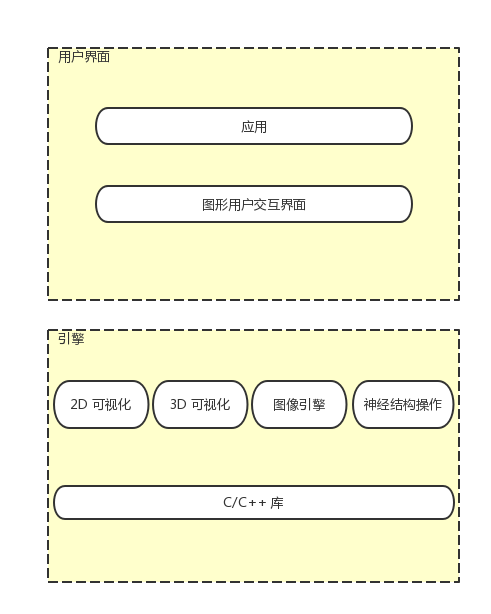
\includegraphics[width=108mm]{images/framework}
\caption{SWC 核心模块}
\label{fan2}
\end{figure}

如图 \ref{fan2} 所示,在 SWC 框架上,我们在 4 个核心模块:2D 可视化,3D 可视化, 图像分析和神经结构实现了图形化用户界面的 neuTube 1.0。

\subsubsection{2D 可视化}

\begin{figure}
\centering
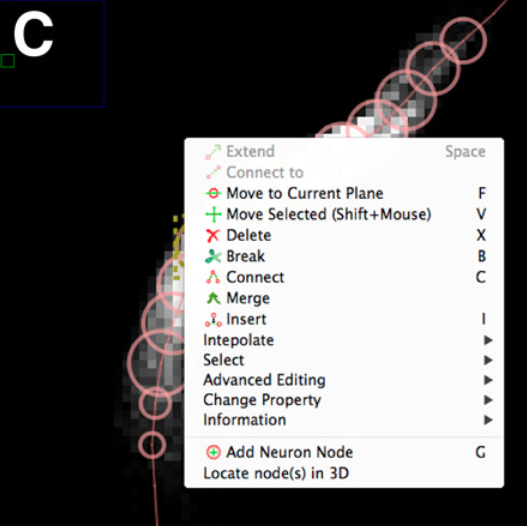
\includegraphics[width=108mm]{images/3b}
\caption{基本几何元素与相关功能}
\label{fan3}
\end{figure}

二维可视化模块提供的显示 3D 图像和神经元结构切片,以及允许用户与 2D 显示交互的功能。这个模块便于用户仔细检查和精确编辑。例如,用户可以放大感兴趣的区域,定位精确跟踪点,或者应用细粒度组件优化神经元结构。2D 可视化的目的是展示重建的结果和数据是否相符而不是现实的神经元结构。如图\ref{fan3} 所示,我们只使用两个几何元素:线和圆圈来代表一个神经元的形态。


二维可视化便于显示恰好在一个平面上的点,但是不适合展示和平面垂直的地方。我们使用两个策略来解决这个问题。首先,为每个被平面穿过的点展示展示一个圆圈。相对应的圆越大,横截面面积越大,这就通过圆的面积告诉用户节点到平面的距离。其次,我们使用颜色来区分一个节点是否在平面上。颜色越饱和,越不透明,节点距离平面越远。着色选项根据用户的反馈和调整的人工调整,然后使用不可变的软件软件参数生成。为了允许用户查看神经元结构的球状结构,我们也将项目整个骨架片视图到一个切片上。

\subsubsection{3D 可视化}
\begin{figure}
\centering
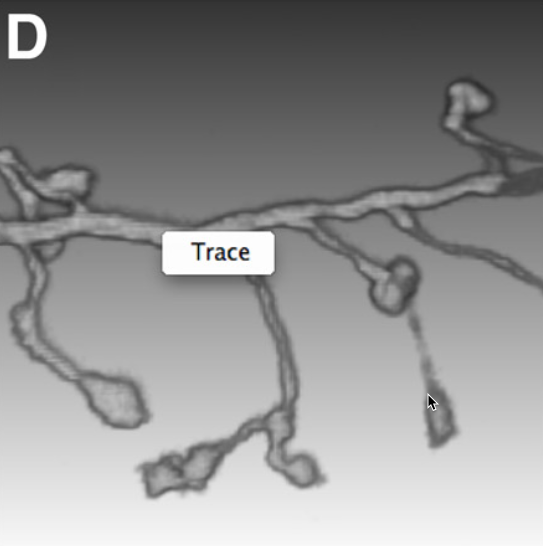
\includegraphics[width=108mm]{images/3d}
\caption{原始图像实时渲染效果}
\label{fan4}
\end{figure}

\begin{figure}
\centering
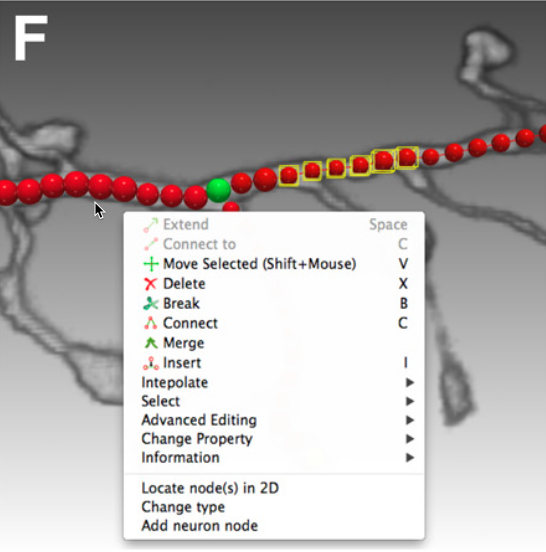
\includegraphics[width=108mm]{images/3f}
\caption{数字重建结果实现渲染效果}
\label{fan5}
\end{figure}

如图 \ref{fan4}、\ref{fan5} 所示,3D 可视化模块是为了实时渲染 3D 图像和神经结构。在 3D 可视化窗口中,用户可以直接展示神经轨迹并编辑,并且任何的改变会同步反映在 2D 可视化窗口中,反之亦然。

\subsubsection{图像分析}
这个模块提供了自动绘制的神经元或神经元分支,允许用户以最小的交互获得神经元结构。例如,用户只需要选择单击分支上的一点便可以选择一个分支。本文之前论述的一个主要改进是用 SWC 框架中定义的树状模型替代了圆柱模型。此外,我们实现了一个基于最短路径方法的用来自动重建的点对点绘制函数。这个函数类似于 Simple Neurite Tracer 和 Vaa3d,但我们可以在 2D 和 3D 同时使用。

\subsubsection{神经结构操作}
\begin{figure}
\centering
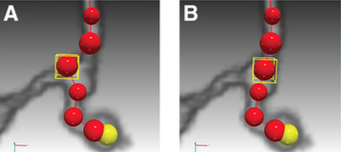
\includegraphics[width=108mm]{images/t6}
\caption{神经结构操作示例1}
\label{fan6}
\end{figure}

\begin{figure}
\centering
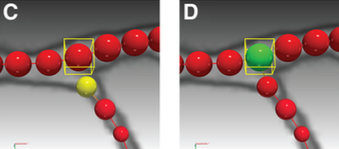
\includegraphics[width=108mm]{images/t7}
\caption{神经结构操作示例2}
\label{fan7}
\end{figure}

\begin{figure}
\centering
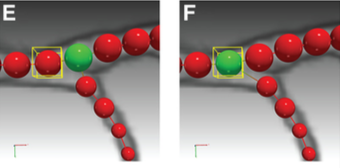
\includegraphics[width=108mm]{images/t8}
\caption{神经结构操作示例3}
\label{fan8}
\end{figure}

\begin{figure}
\centering
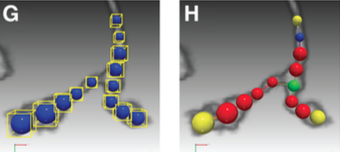
\includegraphics[width=108mm]{images/t9}
\caption{神经结构操作示例4}
\label{fan9}
\end{figure}

\begin{figure}
\centering
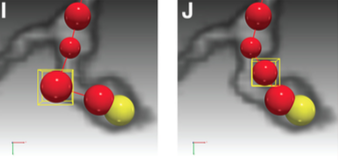
\includegraphics[width=108mm]{images/t10}
\caption{神经结构操作示例5}
\label{fan10}
\end{figure}

\begin{figure}
\centering
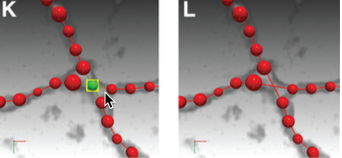
\includegraphics[width=108mm]{images/t11}
\caption{神经结构操作示例16}
\label{fan11}
\end{figure}

这个模块提供了对任意节点的神经结构编辑功能。用户可以通过鼠标点击或键盘快捷键来改变神经结构的几何和拓扑结构。根据前文所述,这个模块将操作分成不同的层次。
为了减轻工作量,我们构建了一下高层次的操作。
插入:在很多情况下,一个神经分支或者一个端分支是足够光滑到用线性结构表示。利用这个性质,如图 \ref{fan6} 所示,可以允许用户快速纠正多个节点的几何属性。
设置分叉点:两段神经元交叉的地方很容易出现分叉点错误的情况。完整的手工纠错包括选择两个节点并将它们合并在一起。设置分叉点的简化了用户的操作,如图 \ref{fan7} 所示,用户只需要创建一个分支点即可。
重置分叉点:这个操作提供了修正一个分支点的另一种方式。在这个操作中,如图 \ref{fan8}所示,用户选择一个节点,程序将尝试移动相邻分支结构到对应节点。程序自动会根据角度自动确定移动哪个分支。
连接多个节点:连接两个接节点是最基本的操作之一,但是仍然需要耐心的完成多个步骤,包括选择节点和触发连接的命令。人工操作的数量会随着节点需要连接的数量增加。为此,如图 \ref{fan9} 所示,neutube 根据两两距离的最小生成树提供了自动连接多个节点的操作。
消除拐角:定义将三个节点依次连接形成的锐角为拐角。中间的节点称为转折点,另外两个节点称为侧节点。如图 \ref{fan10}所示,删除操作是将转折点用两个侧节点差值形成的新节点替代。
消除交叉点:交叉是一种常见的绘制错误,当两个分支在某一点里的很近时。纠正一个分支需要连接和分离多个节点。如图 \ref{fan11}所示,为此我们添加了消除交叉点的操作。

\subsubsection{实现}
软件由 C/C++ 编程语言和多个第三方库编写完成。主要的第三方库是 Qt,Qt 提供了跨平台的 GUI 开发框架。3D 可视化模块建立在 OpenGL 2.0 用 GLSL 编写完成。我们编写高效的生成两种基本几何元素(球和圆柱)的着色器,实现了一个可以快速渲染神经结构的引擎。我们所有的几何基元都有调整不透明度的选项,可以根据可视化的顺序需求生成一个合理的半透明的场景。对于实现渲染复杂的半透明的场景的功能,我们也实现了双深度剥落和加权平均融合算法,这是两种常用的顺序无关的透明算法。这两个算法不需要高端图形卡提供的特殊硬件特性,提供了 neuTube 1.0能够呈现复杂场景的软件可移植性。用户可以根据实际场景,在运行时切换性能更好的算法。
为了在 3D 场景中显示包含了原始图像信息和重建神经信息的图像信号,我们把这些信息作为 3D 文理信息导入到 GPU,并由立体着色器渲染。立体着色器提供了有关立体成分的算法,包括直接体视化,最大密度投影和其不透明变量,局部最大密度投影等。每个算法都有其独特的优点。举例来说最大密度投影允许用户查看通常代表细神经分支的弱信号,直接体视化展示在低噪声下展示大脑结构。用户还可以在 3D 视角下交互式的跟用鼠标单击的方式跟踪。

\section{结果}
我们将 neuTube 1.0 和其他神经重建软件程序(Neuromantic 和 Neurostudio)进行比较,因为这两个软件虽然缺失了一些重要的功能,但仍然是最接近 SWC 框架的两个程序。我们用来自 DIADEM 数据库的4个 3D 图像作为测试材料,让四位用户在相同的时间限制下进行升级结构重建。和真实的应用场景相似,用户在不能分辨或修正错误时停止重建。这个实现反映了软件可视化和编辑功能的灵活程度。我们用包括分支节点和终点等关键节点的准确性来衡量重建结果的准确度。假设共有 N 个节点,其中 M 个节点和真实值匹配,这么重建错误可以用下式表达:
$$Error = \frac{T_d(F_p+F_n) + \sum_{m=1}^{m} d_m}{N}$$

\begin{figure}
\centering
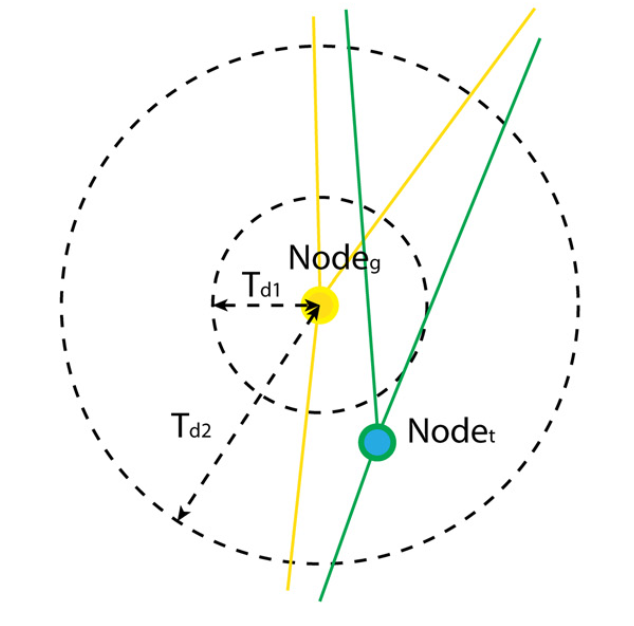
\includegraphics[width=108mm]{images/12}
\caption{匹配点对之间的距离定义}
\label{fan12}
\end{figure}

如图 \ref{fan12} 所示,其中 $F_p$ 和 $F_n$ 是错误的正例和错误的反例的数量,相应的 $T_d$ 代表了匹配点对之间允许的最大距离,$d$ 代表了第 m 个匹配点对之间的的距离。
我们的错误衡量机制基于 DIADEM,但是对于评价神经重建的交互性上有两个主要的修改。一个修改是我们的关键的匹配机制是全局的,而 DIADEM 有一个确定的从根节点开始顺序,这就造成了在上游节点的权重更高。对于用户来说,上游节点的缺失和下游节点的缺失是同等重要的。因此,我们的衡量机制是顺序无关的,所有的节点有同样的权重。另一个不同是我们的衡量机制通过我们之前接受的匹配阈值 ($T_d$) 将拓扑结构错误和位置错误结合起来。这个阈值 $T_d$ 和 DIADEM 中的区域阈值类似,但是我们并不赋予固定的值,而是根据根据主体或者应用来调整。
通过比较各种参数,neuTube 1.0 实现了比 Neuromantic 和 Neurostudio 更高的神经重建准确度。阈值越大 neuTube 1.0 的优势越明显,这显示了 neuTube 1.0 可以帮助用户通过比其他软件更多的关键点来获得更准确的神经结构精度。
}




  }

  \backmatter

  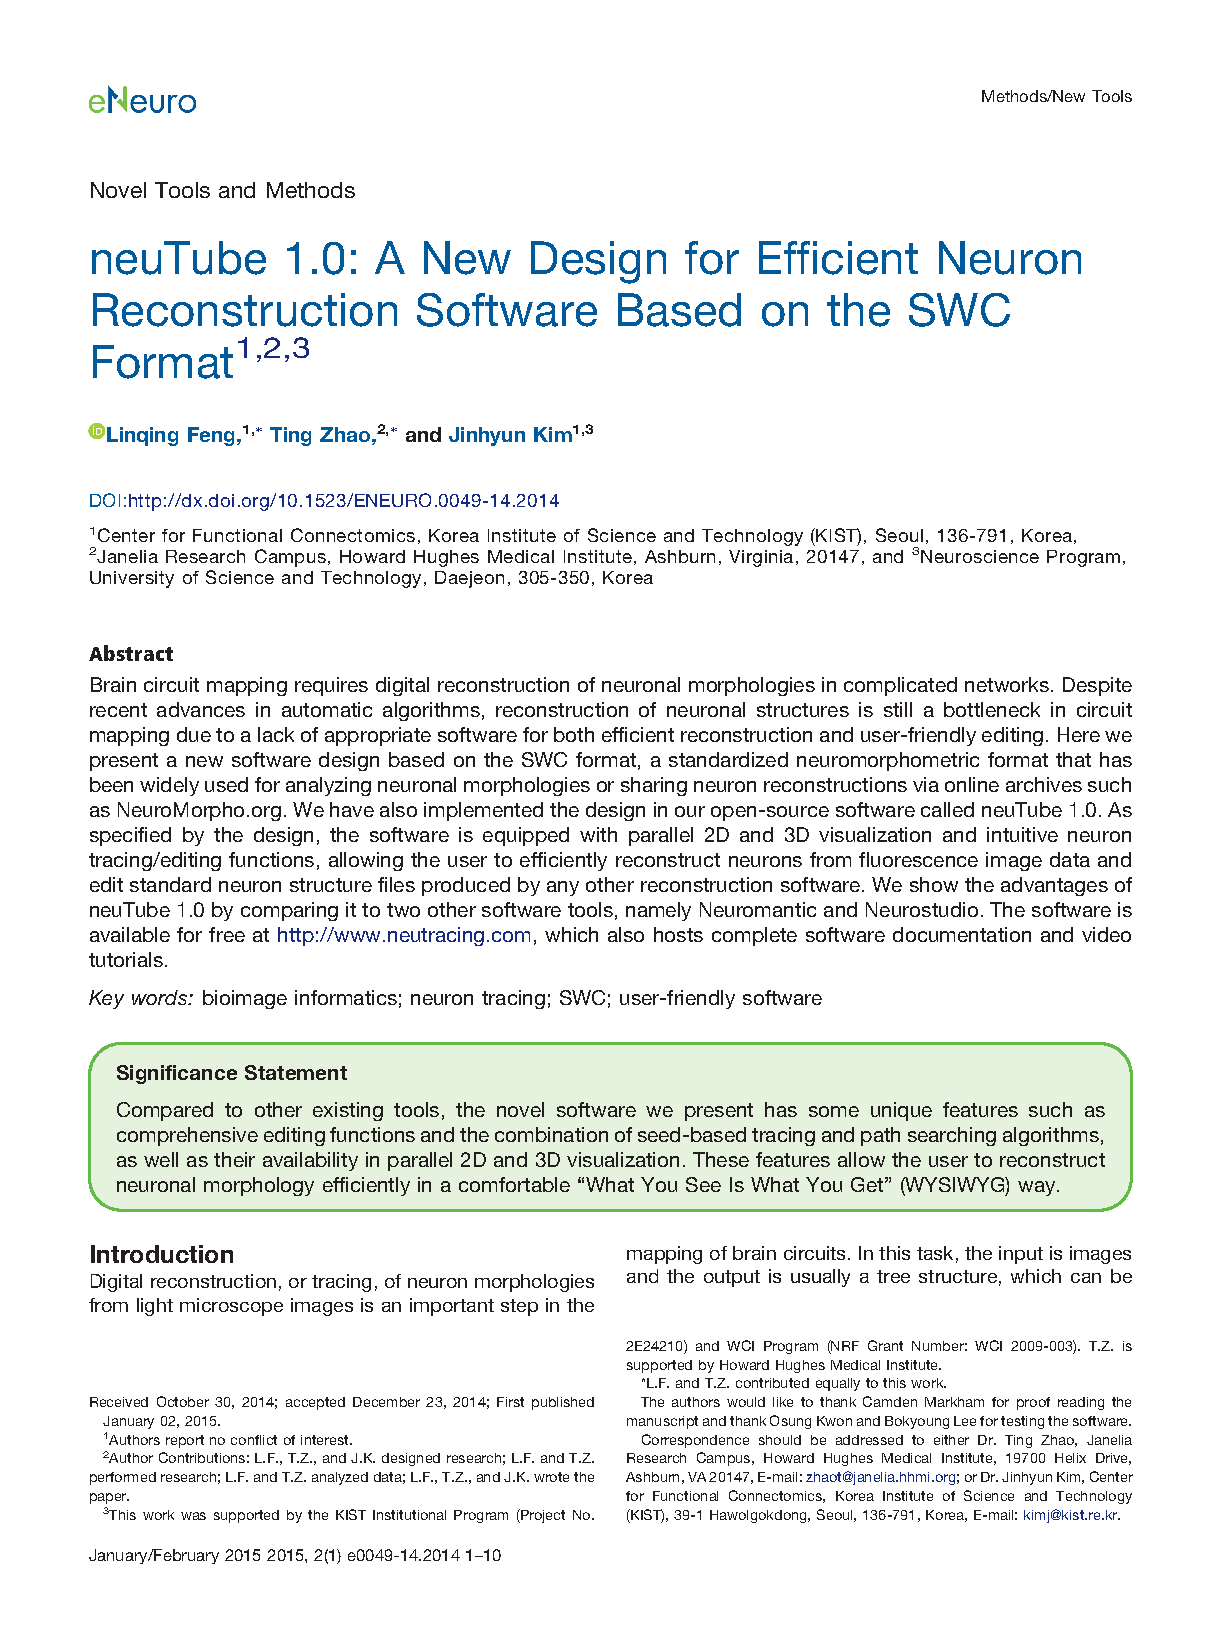
\includepdf[pages=-]{data/waiwenyuanwen.pdf}

\end{document}
